% Options for packages loaded elsewhere
\PassOptionsToPackage{unicode,pdfpagelabels}{hyperref}
\PassOptionsToPackage{hyphens}{url}
\PassOptionsToPackage{dvipsnames,svgnames,x11names}{xcolor}
%
\documentclass[
  12pt,
  a4paper,
]{report}

\usepackage{amsmath,amssymb}
\usepackage{iftex}
\ifPDFTeX
  \usepackage[T1]{fontenc}
  \usepackage[utf8]{inputenc}
  \usepackage{textcomp} % provide euro and other symbols
\else % if luatex or xetex
  \usepackage{unicode-math}
  \defaultfontfeatures{Scale=MatchLowercase}
  \defaultfontfeatures[\rmfamily]{Ligatures=TeX,Scale=1}
\fi
\usepackage{lmodern}
\ifPDFTeX\else  
    % xetex/luatex font selection
\fi
% Use upquote if available, for straight quotes in verbatim environments
\IfFileExists{upquote.sty}{\usepackage{upquote}}{}
\IfFileExists{microtype.sty}{% use microtype if available
  \usepackage[]{microtype}
  \UseMicrotypeSet[protrusion]{basicmath} % disable protrusion for tt fonts
}{}
\makeatletter
\@ifundefined{KOMAClassName}{% if non-KOMA class
  \IfFileExists{parskip.sty}{%
    \usepackage{parskip}
  }{% else
    \setlength{\parindent}{0pt}
    \setlength{\parskip}{6pt plus 2pt minus 1pt}}
}{% if KOMA class
  \KOMAoptions{parskip=half}}
\makeatother
\usepackage{xcolor}
\usepackage[top=2cm,bottom=2cm,left=1.5cm,right=1.5cm,marginparsep=2cm]{geometry}
\setlength{\emergencystretch}{3em} % prevent overfull lines
\setcounter{secnumdepth}{5}
% Make \paragraph and \subparagraph free-standing
\makeatletter
\ifx\paragraph\undefined\else
  \let\oldparagraph\paragraph
  \renewcommand{\paragraph}{
    \@ifstar
      \xxxParagraphStar
      \xxxParagraphNoStar
  }
  \newcommand{\xxxParagraphStar}[1]{\oldparagraph*{#1}\mbox{}}
  \newcommand{\xxxParagraphNoStar}[1]{\oldparagraph{#1}\mbox{}}
\fi
\ifx\subparagraph\undefined\else
  \let\oldsubparagraph\subparagraph
  \renewcommand{\subparagraph}{
    \@ifstar
      \xxxSubParagraphStar
      \xxxSubParagraphNoStar
  }
  \newcommand{\xxxSubParagraphStar}[1]{\oldsubparagraph*{#1}\mbox{}}
  \newcommand{\xxxSubParagraphNoStar}[1]{\oldsubparagraph{#1}\mbox{}}
\fi
\makeatother


\providecommand{\tightlist}{%
  \setlength{\itemsep}{0pt}\setlength{\parskip}{0pt}}\usepackage{longtable,booktabs,array}
\usepackage{calc} % for calculating minipage widths
% Correct order of tables after \paragraph or \subparagraph
\usepackage{etoolbox}
\makeatletter
\patchcmd\longtable{\par}{\if@noskipsec\mbox{}\fi\par}{}{}
\makeatother
% Allow footnotes in longtable head/foot
\IfFileExists{footnotehyper.sty}{\usepackage{footnotehyper}}{\usepackage{footnote}}
\makesavenoteenv{longtable}
\usepackage{graphicx}
\makeatletter
\def\maxwidth{\ifdim\Gin@nat@width>\linewidth\linewidth\else\Gin@nat@width\fi}
\def\maxheight{\ifdim\Gin@nat@height>\textheight\textheight\else\Gin@nat@height\fi}
\makeatother
% Scale images if necessary, so that they will not overflow the page
% margins by default, and it is still possible to overwrite the defaults
% using explicit options in \includegraphics[width, height, ...]{}
\setkeys{Gin}{width=\maxwidth,height=\maxheight,keepaspectratio}
% Set default figure placement to htbp
\makeatletter
\def\fps@figure{htbp}
\makeatother

\usepackage{geometry}       % Control page margins
\usepackage{setspace}       % Custom line spacing
\usepackage{titlesec}       % Modern section titles
\usepackage{amsmath}        % Math environments
\usepackage{amssymb}        % Math symbols
\usepackage{amsfonts}       % Math fonts
\usepackage{mathtools}      % Extra math tools
\usepackage{physics}        % For partial derivatives
\usepackage{siunitx}        % SI units
\sisetup{per-mode = symbol} % Set SI unit fractions to use a solidus
\usepackage{commath}        % For derivatives

\usepackage{graphicx}       % For including images
\usepackage{xcolor}         % Color text, if needed
\usepackage{xparse}
\usepackage{booktabs}       % Improved tables
\usepackage{enumitem}       % Customized lists
\usepackage{float}          % Improved figure placement
\usepackage{tikz}           % Core TikZ package
\usetikzlibrary{positioning, arrows.meta, external}
\usepackage{circuitikz}     % For circuits!
\usepackage{pgfplots}       % For plots
\pgfplotsset{compat=1.18}   % Set compatibility to 1.18
\tikzexternalize[prefix=tikz/] % Save tikz figures to a folder
\tikzset{external/up to date check=md5} % Check for changes using md5
\usepackage{fancyhdr}       % Customize headers and footers
\usepackage{appendix}       % Appendices
\usepackage{cancel}         % Cancel terms in equations
\usepackage{tcolorbox}
\usepackage{mdframed}       % Framed text blocks
\usepackage{subfiles}       % Subfiles package
% Document navigation
\usepackage[pdfpagelabels]{hyperref}       % For clickable links and cross-references
\usepackage{bookmark}       % Improved bookmarks for navigation
\AtBeginDocument{\RenewCommandCopy\qty\SI}
% spacing and margins
\onehalfspacing%
% \geometry{%
%     a4paper,
%     left=1.5cm,
%     right=1.5cm,
%     top=2cm,
%     bottom=2cm
% }
\setlength{\marginparwidth}{2cm}
% Header and footer settings
\fancypagestyle{plain}{%
  \fancyhf{}%
  \fancyhead[L]{\textbf{Nicholas Russell}}%
  \fancyhead[C]{ELECTENG 332: Control Systems Notes}%
  \fancyhead[R]{August 10th, 2024}%
  \fancyfoot[R]{\thepage}%
  \renewcommand{\headrulewidth}{0.4pt}%
  \renewcommand{\footrulewidth}{0pt}%
}
\setlength{\headheight}{16.5pt}
\titleformat{\chapter}[display]
  {\normalfont\LARGE\bfseries}{\textcolor{blue}{Module {\thechapter}:}}{1pt}{}
\titleformat{\section}
  {\normalfont\Large\bfseries}{\thesection}{1em}{}
\titlespacing*{\chapter}{0pt}{20pt}{10pt}
\titlespacing*{\part}{0pt}{20pt}{10pt}
\titlespacing*{\section}{0pt}{20pt}{10pt}
\renewcommand{\theequation}{\arabic{equation}}
\title{ELECTENG 332 Notes}
\author{Nicholas Russell}
\setcounter{tocdepth}{3}
% Define colors
\definecolor{borderblue}{HTML}{0099FF} % #0099FF
\definecolor{boxheadcol}{HTML}{D6D6F0} % #D6D6F0
\definecolor{boxbodycol}{HTML}{EBEBF7} % #EBEBF7
% Custom macros
\DeclareSIUnit{\rads}{\radian\per\second}
\newcommand{\bluetext}[1]{\textcolor{blue}{#1}}
\newcommand{\redtext}[1]{\textcolor{red}{#1}}

\makeatletter
\@ifpackageloaded{bookmark}{}{\usepackage{bookmark}}
\makeatother
\makeatletter
\@ifpackageloaded{caption}{}{\usepackage{caption}}
\AtBeginDocument{%
\ifdefined\contentsname
  \renewcommand*\contentsname{Table of contents}
\else
  \newcommand\contentsname{Table of contents}
\fi
\ifdefined\listfigurename
  \renewcommand*\listfigurename{List of Figures}
\else
  \newcommand\listfigurename{List of Figures}
\fi
\ifdefined\listtablename
  \renewcommand*\listtablename{List of Tables}
\else
  \newcommand\listtablename{List of Tables}
\fi
\ifdefined\figurename
  \renewcommand*\figurename{Figure}
\else
  \newcommand\figurename{Figure}
\fi
\ifdefined\tablename
  \renewcommand*\tablename{Table}
\else
  \newcommand\tablename{Table}
\fi
}
\@ifpackageloaded{float}{}{\usepackage{float}}
\floatstyle{ruled}
\@ifundefined{c@chapter}{\newfloat{codelisting}{h}{lop}}{\newfloat{codelisting}{h}{lop}[chapter]}
\floatname{codelisting}{Listing}
\newcommand*\listoflistings{\listof{codelisting}{List of Listings}}
\makeatother
\makeatletter
\makeatother
\makeatletter
\@ifpackageloaded{caption}{}{\usepackage{caption}}
\@ifpackageloaded{subcaption}{}{\usepackage{subcaption}}
\makeatother

\ifLuaTeX
  \usepackage{selnolig}  % disable illegal ligatures
\fi
\usepackage{bookmark}

\IfFileExists{xurl.sty}{\usepackage{xurl}}{} % add URL line breaks if available
\urlstyle{same} % disable monospaced font for URLs
\hypersetup{
  pdftitle={ELECTENG 332 Notes},
  pdfauthor={Nicholas Russell},
  colorlinks=true,
  linkcolor={blue},
  filecolor={Maroon},
  citecolor={Blue},
  urlcolor={Blue},
  pdfcreator={LaTeX via pandoc}}


\author{}
\date{}

\begin{document}

\begin{titlepage}
    \centering
    
\includegraphics[width=0.8\textwidth]{images/DECSE-HC-4C-01.png}\\[1cm]
    {\LARGE \textbf{ELECTENG 332}}\\[0.5cm]
    {\Large Notes on Control Systems}\\[0.5cm]
    {\textit{Dear god help me, not another one\dots\ }}\\[2cm]
    {\large by}\\[0.3cm]
    {\large \textbf{Nicholas Russell}}\\[1.4cm]
    {\large August 10th, 2024}
    \vfill
    {\large Department of Electrical, Computer, and Software Engineering}\\[0.3cm]
    {\large Faculty of Engineering}\\[0.3cm]
    {\large University of Auckland}
\end{titlepage}

\renewcommand*\contentsname{Table of contents}
{
\hypersetup{linkcolor=}
\setcounter{tocdepth}{2}
\tableofcontents
}

\bookmarksetup{startatroot}

\chapter*{Introduction}\label{introduction}
\addcontentsline{toc}{chapter}{Introduction}

\markboth{Introduction}{Introduction}

These notes are compiled from the lectures of ELECTENG 332: Signals and
Systems at The University of Auckland. They are intended as a personal
reference to assist with assignments, exam preparation, and
understanding key concepts in control systems and signal analysis.

The notes cover various topics, including signal modeling, feedback
systems, and time-domain analysis, which are crucial for the analysis
and design of control systems. Feel free to add personal insights or
additional references as you study these materials.

\bookmarksetup{startatroot}

\chapter*{Organisation of the Notes}\label{organisation-of-the-notes}
\addcontentsline{toc}{chapter}{Organisation of the Notes}

\markboth{Organisation of the Notes}{Organisation of the Notes}

The notes are divided into modules, with each section corresponding to
specific topics covered in the course. Here's how they are organized:

\begin{itemize}
\item
  \textbf{Module 1: Basics of Signals and Systems}\\
  Key topics include time-domain representation, Laplace transforms, and
  system responses.
\item
  \textbf{Module 2: Mathematical Modeling of Dynamic Systems}\\
  Covers the mathematical modeling of electrical and mechanical systems
  using block diagrams and differential equations.
\item
  \textbf{Module 3: Block Diagrams \& Feedback Systems Overview}\\
  Discusses the fundamentals of feedback control, including system
  stability, noise reduction, and transient response characteristics.
\item
  \textbf{Module 4: Time Domain Analysis of Linear Systems}\\
  Provides a detailed analysis of transient and steady-state responses,
  including rise time, settling time, and peak overshoot.
\item
  \textbf{Module 5: Stability Analysis of Linear Systems}\\
  Focuses on analyzing the stability of linear systems using different
  criteria such as the Routh-Hurwitz criterion.
\end{itemize}

\bookmarksetup{startatroot}

\chapter*{How I Use These Notes}\label{how-i-use-these-notes}
\addcontentsline{toc}{chapter}{How I Use These Notes}

\markboth{How I Use These Notes}{How I Use These Notes}

These notes are a living document that I update as I gain a deeper
understanding of the material. Here's how I use them:

\begin{itemize}
\tightlist
\item
  \textbf{Quick Reference}: For quick lookups, the Table of Contents
  helps navigate directly to the relevant section.
\item
  \textbf{In-Depth Study}: For exam preparation, I revisit each module,
  ensuring I understand each concept before moving on.
\item
  \textbf{Personal Insights}: I add thoughts, extra readings, and
  questions for further study.
\end{itemize}

Exercises and examples are included to enhance the understanding of more
complex topics, such as feedback control and stability analysis.

\part{Module 1}

\chapter{Basics of Signals and
Systems}\label{basics-of-signals-and-systems}

\phantomsection\label{learningoutcomesmodule1}
\section*{Learning Outcomes}\label{learning-outcomes}
\addcontentsline{toc}{section}{Learning Outcomes}

\markright{Learning Outcomes}

\begin{enumerate}[label=\(\blacktriangleright\), leftmargin=*, itemsep=0.5em]
    \item Uniqueness of the Exponential Signal
    \item Concept of Engineering Infinity
    \item Concept of Complex Frequency
    \item Classification of Signals: Energy \& Power
    \item Classification of Systems
    \item What is a Control System
    \item Classification of a Control System: Open-loop \& Closed-loop
\end{enumerate}

\chapter{Topic 1: The Importance of the Exponential
Function}\label{topic-1-the-importance-of-the-exponential-function}

\phantomsection\label{topic1}
The Exponential function, written as either \(e^{ax}\) or \(e^{at}\)
depending on whether it is \(f(t)\) or \(f(x)\), has properties that
make it mathematically unique.

\begin{enumerate}
\def\labelenumi{\arabic{enumi}.}
\item
  The derivative (rate of change) of the exponential function is the
  exponential function itself. More generally, this is a function whose
  rate of change is proportional to the function itself.

  \phantomsection\label{exp-derivative}
  \begin{equation} 
  \label{eq:exp-derivative}     
  \dv{e^{ax}}{x} = a e^{ax} 
  \end{equation}
\item
  The integral of the exponential function is also the exponential
  function itself.

  \phantomsection\label{exp-integral}
  \begin{equation} 
  \label{eq:exp-integral}     
  \int e^{ax} \dd{x} = \frac{1}{a} e^{ax} 
  \end{equation}
\end{enumerate}

\phantomsection\label{topic2}
\chapter{Topic 2: The Concept of Engineering
Infinity}\label{topic-2-the-concept-of-engineering-infinity}

Consider a signal \(e^{-at}\). The time constant for this signal is
\(T = \frac{1}{a}\). Theoretically, the signal is meant to decay to zero
as time approaches infinity, i.e.

\phantomsection\label{engineering-infinity}
\begin{equation} 
\label{eq:eng-infinity}     
\lim_{t \to \infty} e^{-at} = 0  
\end{equation}

But in practice, this is not the case, as its value will be very, very
small after five time constants \(5T\) (or \(5\tau\)). This is the
\textcolor{red}{\textbf{\textit{Concept of Engineering Infinity}}}. The
signal will never reach zero, but it will be so small that it can be
considered zero for all practical purposes. This is a very important
concept in control systems, as it allows us to simplify our calculations
and analysis.

\chapter{Topic 3: The Concept of Complex
Frequency}\label{topic-3-the-concept-of-complex-frequency}

\phantomsection\label{topic3}
Complex frequency is found commonly in electrical engineering. It is
often notated as \(j\omega\) or \(s = \sigma \pm j\omega\). These
frequencies always come in pairs, so the use of \(\pm\) is implicit to
this, as complex numbers have complex conjugates (normally notated by
\(z^*\) or \(\bar{z}\)). i.e.~\(s = \sigma + j\omega\) has the conjugate
\(s=\sigma - j\omega\).

\phantomsection\label{argand-figure}
\begin{figure}

{\centering 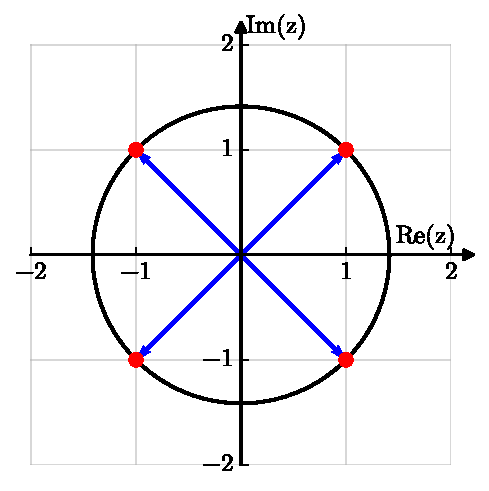
\includegraphics{chapters/module1/topic3_comp_freq_files/figure-pdf/argand-output-1.pdf}

}

\caption{Argand diagram of \(|z| = \sqrt{2}\)}

\end{figure}%

\phantomsection\label{de-moivre-formula}
This is also backed up by De Moivre's formula which is defined
mathematically as:

\begin{gather}
    \label{eq:de-moivre-formula}
    \forall x \in \mathbb{R}, \quad \forall n \in \mathbb{Z}, \\
    e^{jnx} = \cos(n x) + j \sin(n x)  
\end{gather}

\phantomsection\label{de-moivre-formula-general}
Or more generally for our applications (this is also known as Euler's
formula):

\begin{gather}
    \label{eq:de-moivre-formula-general}
    e^{jx} = \cos(x) + j \sin(x) \\
    \text{Where} \, x \in \mathbb{R}\, \text{(\(x\) is real)} \\
    \text{and} \, j \equiv i = \sqrt{-1}
\end{gather}

\phantomsection\label{complex-sinusoid-def-1}
This means that:\\
\begin{mdframed}
    \begin{center}
        \redtext{\emph{A complex frequency \(j\omega \) represents a pure sinusoidal signal of frequency \(\omega \) \unit{\rads}}}
    \end{center}
\end{mdframed}

For example, if a signal has a complex frequency
\(\complexqty[output-complex-root=j, complex-root-position=before-number]{314i}{\rads}\),
then this responds to a pure sinusoid of frequency \(\qty{314}{\rads}\)
(i.e.~\(\qty{50}{\hertz}\)).

\phantomsection\label{exp-damped-sinusoid-def}
Furthermore:\\
\begin{mdframed}
    \begin{center}
        \redtext{\emph{A complex frequency \(s = \sigma + j\omega\) represents an exponentially damped signal of frequency \(j\omega\) \unit{\rads}, and decays/amplifies at a rate decided by \(\sigma\).}}
    \end{center}
\end{mdframed}

For example, the signal \(f(t) =  e^{-10t} \sin(40\pi t)\) would look
like this:




\end{document}
